
\section{Introduction}
\label{sec:intro}
In the era of Big Data, interactive data exploration tools arise as an important mean to explore and derive insights from data through visualization.  
However, perceived interesting patterns in visual data representations, such as relationships or trends, may emerge from irrelevant random effects inherent to the data, such as random noises, large variances, insufficient samples, and biases. 
Without proper statistical control, users may mistake a distinct or dominant visual observation as statistically significant.  
On the other hand, systems that search and recommend visualizations automatically based on such interesting visual features further increase the chance of bogus insights.  
A recent study highlights these issues and shows that visualization and recommendation systems that do not consider the risk of false discovery, such as Vizdom~\cite{vizdom}, SeeDB~\cite{seedb} and Data Polygamy~\cite{polygamy}, become difficult to derive insights safely on real-world datasets \cite{binnig2017sustainable}.

False discovery due to random noise is pervasive in visual data exploration on real-world datasets. For example, when using Vizdom~\cite{vizdom} to explore a recently conducted survey on personal habits and opinions~\cite{binnig2017sustainable}, we observed that the preference on watching films on DVD produced visually different proportions of belief in aliens, as shown in Figure~\ref{fig:example} (A and B).
Just by visually examining these charts, users often falsely assumed that people who prefer to watch movies on DVD are more prone to believe in aliens even though this effect is not statistically significant.
%But such predictor proved neither much sensible nor statistically significant.  

Such observation-based hypotheses may be accumulated quickly as the user continues to explore a dataset, and hence dramatically raises the risk of spurious findings. 
With the same survey dataset, after searching through a few different comparisons we stumbled upon a visualization that suggests hair color predicts whether one knows about Michael Stonebraker, and it would be statistically significant if considered as a lone hypothesis. This phenomenon is often referred to as data dredging or $p$-hacking~\cite{head2015extent}, and formally known as the multiple comparison problem~\cite{shaffer1995multiple}.

Several challenges exist to control false insights in such interactive data exploration.  
The first question is what could even be considered as a hypothesis in visual data exploration.
In some cases users might explicitly specify certain hypotheses, but in other instances they do not formulate any hypothesis but still use visualization to infer about the data or to extract an insight.
An ideal system should assist users in hypothesis formulation and corresponding hypothesis test selection.

Second, interactive data exploration mandates that hypotheses are formulated dynamically based on the process of human decision making.  
However the classical statistical procedures such as Bonferroni~\cite{bonferroni1936teoria} and Sequential FDR~\cite{g2016sequential} are not dynamic as they require collecting all the hypotheses a priori before finalizing any significance result.  
Moreover these traditional techniques assume complete pass of the dataset, and thus would make the system non-interactive on larger data.  
Thus an ideal system for interactive control of false discovery should follow progressive computation, which proves to be a more appealing paradigm~\cite{zgraggen2016progressive, onlineagg}.  

Finally, parts of the data exploration process can be automated through algorithmic search and recommendation. Such automatic data exploration should also be subject to false discovery control.  

In this demo, we present \system{}\footnote{\system{} stands for Quantifying the Uncertainty in Data Exploration.}, a first ``safe'' visual data exploration tool that addresses these challenges. 
In \system{}, we therefore implemented recent techniques in interactive false discovery control that are both dynamic and progressive~\cite{zhao2016controlling}, apply them to visual data exploration and visualization recommendation, and expose them through a pen- \& touch-based user interface that simplifies and in some cases even automates the creation of hypothesis tests.


%Thus, to address theses challenges, we implemented the recent advance in interactive false discovery control that is both dynamic and progressive, and applied to both visual data exploration and recommendation~\cite{zhao2016controlling}. 

\begin{figure}
\centering
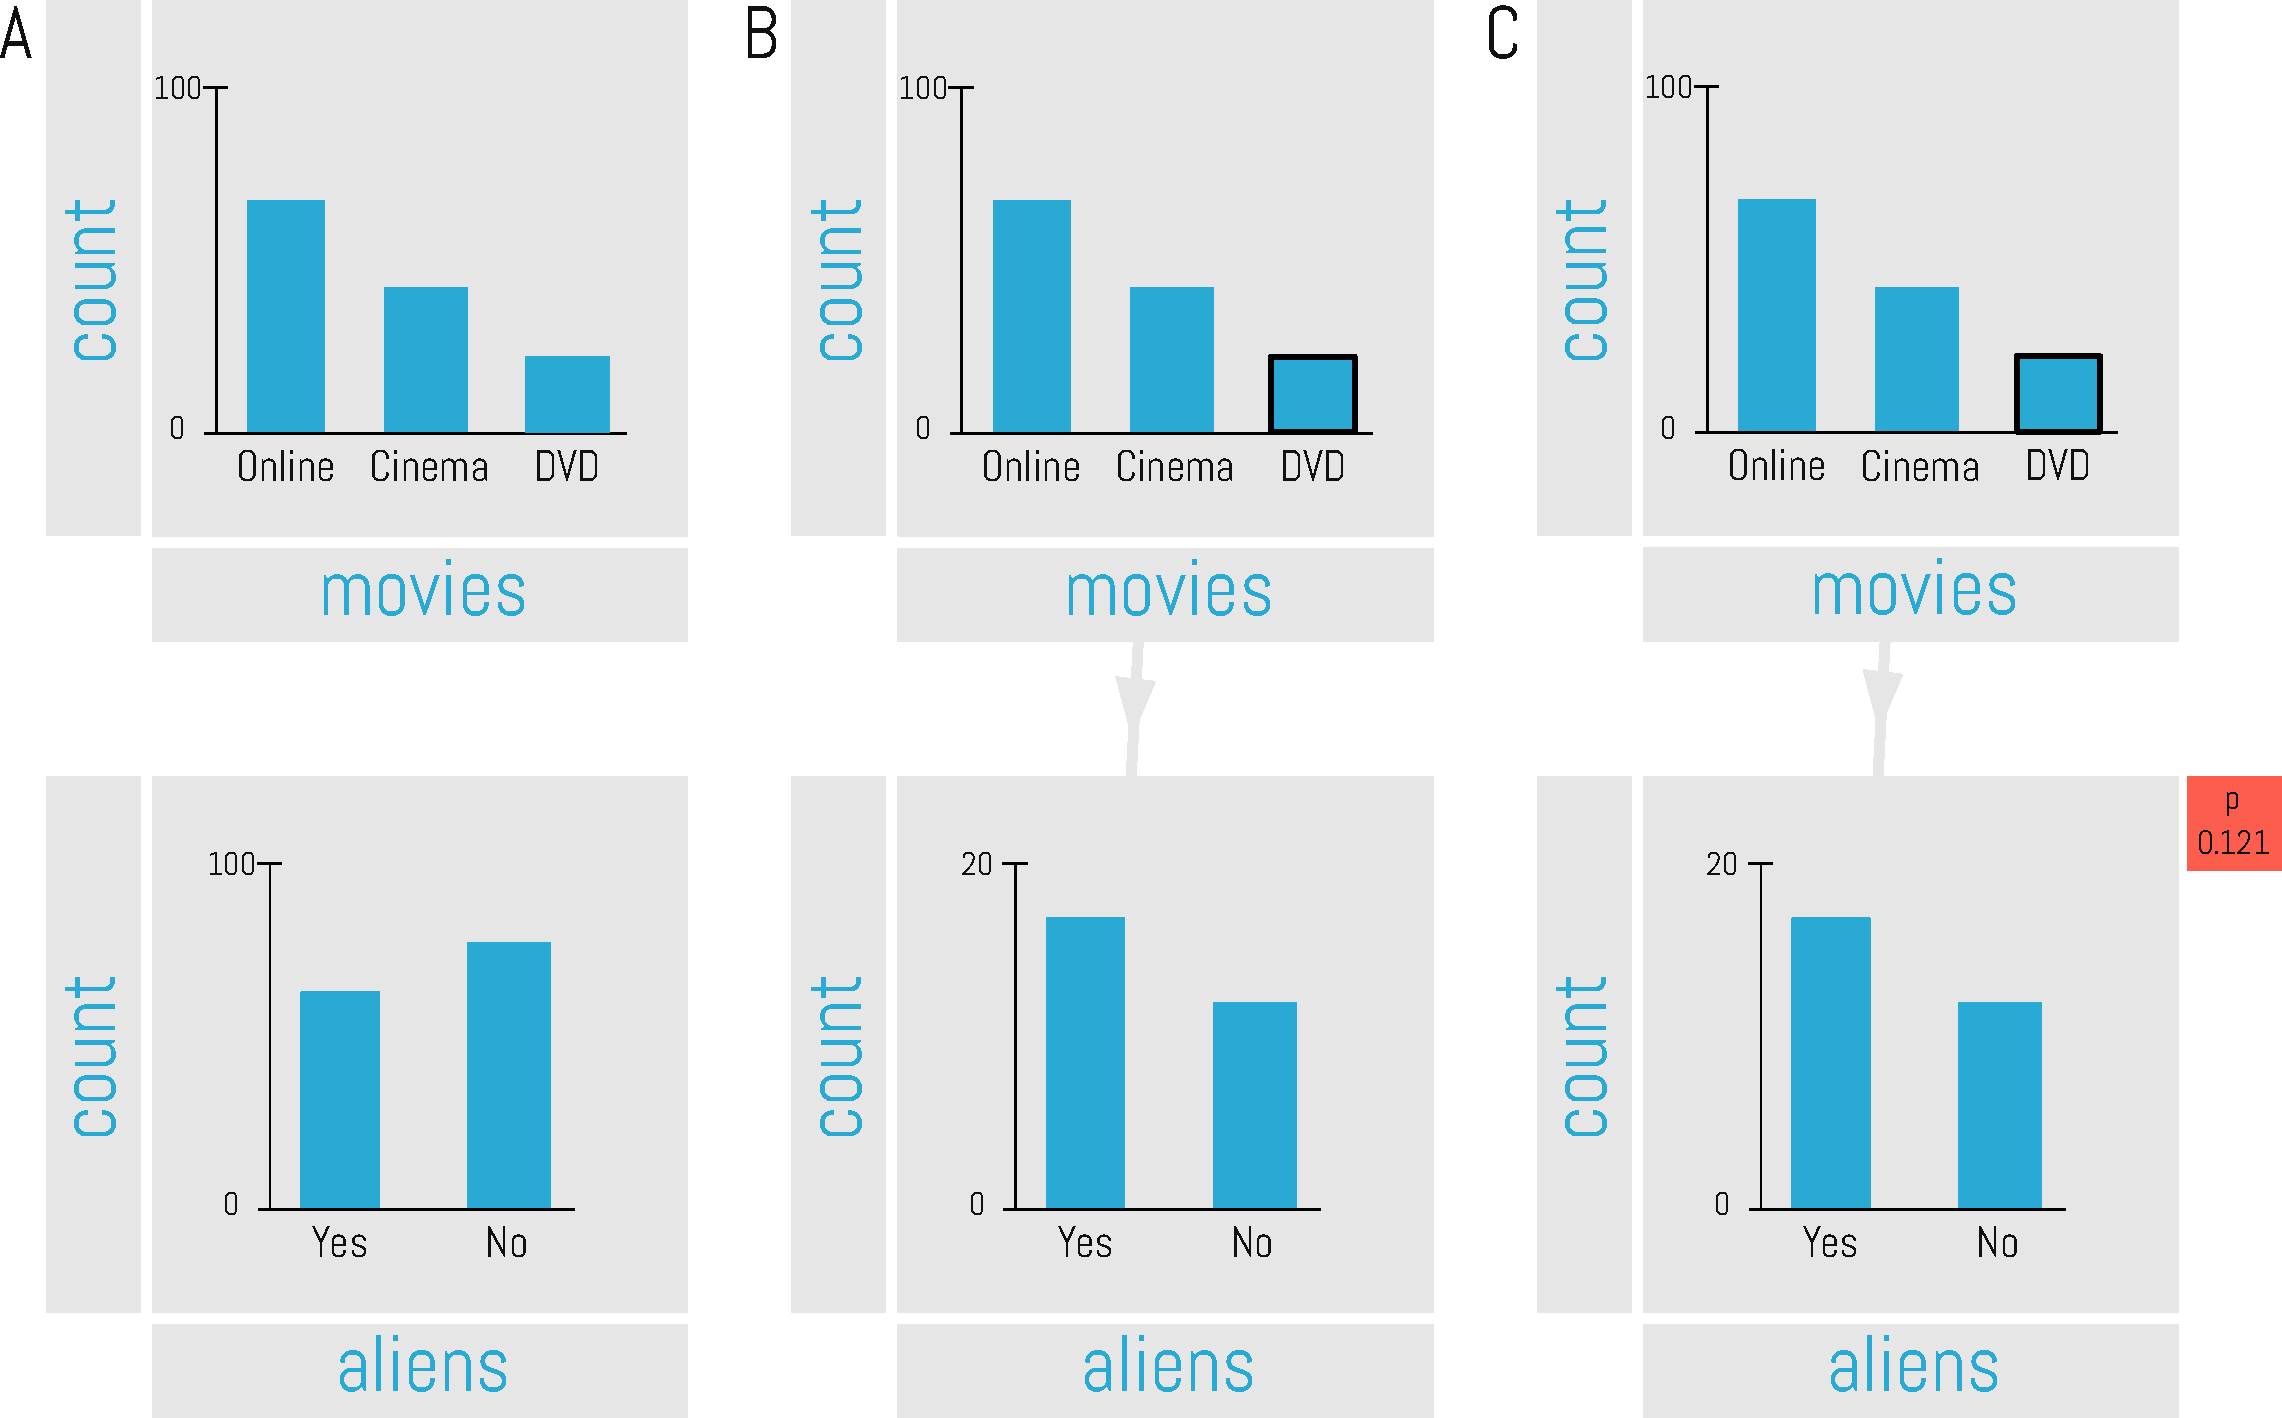
\includegraphics[width=0.47\textwidth]{figures/example}
\caption{Example of a visualization network where users might be led to false discoveries without automatic hypothesis formulation. (A) two separate visualizations showing preferences for watching movies and how many people believe in alien existence; (B) the two visualizations combined where the bottom one shows proportions of belief in alien existence for only people who like to watch movies on DVD, displaying a noticeable difference compared to the overall population. (C) same visualizations as before but now with automatic hypothesis formulation turned on, highlighting that the observed effect is not statistically significant.}
\label{fig:example}
\vspace{-3.5ex}
\end{figure}